\documentclass{article}

% if you need to pass options to natbib, use, e.g.:
%     \PassOptionsToPackage{numbers, compress}{natbib}
% before loading neurips_2018

% ready for submission
% \usepackage{neurips_2018}

% to compile a preprint version, e.g., for submission to arXiv, add add the
% [preprint] option:
    \usepackage[preprint]{neurips_2018}

% to compile a camera-ready version, add the [final] option, e.g.:
     % \usepackage[final]{neurips_2018}

% to avoid loading the natbib package, add option nonatbib:
    % \usepackage[nonatbib]{neurips_2018}

\usepackage[utf8]{inputenc} % allow utf-8 input
\usepackage[T1]{fontenc}    % use 8-bit T1 fonts
\usepackage{graphicx}
\usepackage[font=small,labelsep=period]{caption}
\usepackage{subfigure}
\usepackage{hyperref}       % hyperlinks
\usepackage{url}            % simple URL typesetting
\usepackage{booktabs}       % professional-quality tables
\usepackage{amsfonts}       % blackboard math symbols
\usepackage{nicefrac}       % compact symbols for 1/2, etc.
\usepackage{microtype}      % microtypography
\usepackage{pifont}
\usepackage{enumerate}
\usepackage{amsmath}
\usepackage{enumitem}
\setlist[enumerate,1]{label=(\arabic*),font=\textup,
leftmargin=7mm,labelsep=1.5mm,topsep=0mm,itemsep=-0.8mm}
\usepackage{algorithm}
\usepackage{algpseudocode}
\usepackage{booktabs}
\renewcommand{\algorithmicrequire}{\textbf{Input:}}  % Use Input in the format of Algorithm
\renewcommand{\algorithmicensure}{\textbf{Output:}} % Use Output in the format of Algorithm
\newcommand{\topcaption}{\setlength{\abovecaptionskip}{0pt} \setlength{\belowcaptionskip}{10pt} \caption}


\title{Detecting Adversarial Examples via Undercover Attack}

% The \author macro works with any number of authors. There are two commands
% used to separate the names and addresses of multiple authors: \And and \AND.
%
% Using \And between authors leaves it to LaTeX to determine where to break the
% lines. Using \AND forces a line break at that point. So, if LaTeX puts 3 of 4
% authors names on the first line, and the last on the second line, try using
% \AND instead of \And before the third author name.

\author{%
  Qifei Zhou \\ %\thanks{}
  School of Software and Microelectronics\\
  Peking University\\
  Beijing 100871, China \\
  \texttt{qifeizhou@pku.edu.cn} \\
  % examples of more authors
  \And
  Weiping Li \\
  School of Software and Microelectronics\\
  Peking University\\
  Beijing 100871, China \\
  \texttt{wpli@ss.pku.edu.cn} \\
  \AND
  Tong Mo \\
  School of Software and Microelectronics\\
  Peking University\\
  Beijing 100871, China \\
  \texttt{motong@ss.pku.edu.cn} \\
  \And
  Yue Wu \\
  Logistics Engineering \\
  University of Science and Technology Beijing \\
  Beijing 100083, China \\
  \texttt{869216739@qq.com} \\
  % \And
  % Coauthor \\
  % Affiliation \\
  % Address \\
  % \texttt{email} \\
}

\begin{document}
% \nipsfinalcopy is no longer used

\maketitle

\begin{abstract}

\end{abstract}

\section{Introduction}

Deep nerual networks (DNNS) are vulneralbe to adverisarial examples \cite{Szegedy2013Intriguing,Goodfellow2014Explaining,Papernot2016Transferability}, imperceptible modifications to the original inputs of a DNN classifier can cause the model to produce incorrect labels. This problem is especially important in safety-critical applications such as self-driving cars. To illustrate how adversarial samples make a system based on DNNs vulnerable, consider the following 
images \ref{car}:

\begin{figure}[h]
  \centerline{
    \subfigure[prohibition sign]{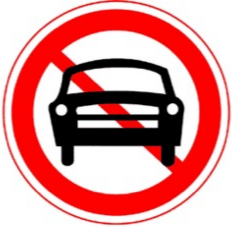
\includegraphics[scale=0.3]{car.png}}
    \subfigure[fire sign]{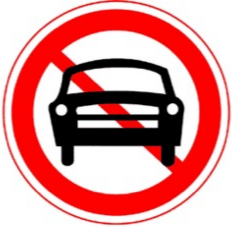
\includegraphics[scale=0.3]{car.png}}
  }
  \caption{(a) is the original image of a prohibition sign}
  \label{car}
\end{figure}

To humans, these two images look the same: we identify each of them as a prohibition sign. The image on the left is indeed an ordinary image of a prohibition sign. We produced the image on the right by adding a very small perturbation that forces a particular DNN to classify it as a fire sign. The work or Kurakin et al. \cite{Kurakin2016Adversarial} showed that these transformations are effective in the physical world. Here, someone with ulterior motives can make self-driving cars behave dangerously taking advantage of the vulnerability of DNNs.

There are quite a few methods have been proposed to fool the model, such as L-BFGS \cite{Szegedy2013Intriguing}, FGSM \cite{Goodfellow2014Explaining}, BIM \cite{Kurakin2016Adversarial}, JSMA \cite{papernot2016the} and C\&W \cite{Carlini2016Towards}. This problem has aroused great concern in the academic world. Many researchers has being trying to explain adversarial examples and find new ways to defend aganist these attack methods. There are numerous defense techniques including image compression or filtering \cite{das2017keeping,xu2018feature}, defensive distillation \cite{papernot2016distillation} and many defenses summarized as Gradient masking \cite{Papernot2016Transferability} or Obfuscated Gradients \cite{athalye2018obfuscated}. Unfortunately, none of these defenses is yet completely satisfactory, they can generally be evaded by stronger attacks wholly or partially. The most popular defense in current research papers is probably adversarial training proposed by Goodfellow et al. \cite{Goodfellow2014Explaining} which also helps us a lot in \emph{Undercover Attack}.

Due to the challenge of defenses, many recent work has turned to detect adversarial examples. Xu et al. used feature squeezing to detect, while such detectors may work well against certain attacks, detectors in this category have been shown to fail in the white box case, where the attacker is aware of the detector \cite{He2017Adversarial}. Feinman et al. \cite{feinman2017detecting} showed that Kernel Density estimates and Bayesian Uncertainty estimates can detect points lie in low-confidence regions of the input space. Pang et al. \cite{pang2018towards} proposed a new loss function named Reverse Cross-entropy which can improve the performance of KD and BU. Howerver, KD and BU have been debeated by C\&W in \cite{carlini2017adversarial} who showed that incorporating kernel density into the objective function makes detection substantially more difficult. Ma et al. \cite{ma2018characterizing} proposed Local Intrinsic Dimensionality which is claimed robust to C\&W and achieves quite execellent performance on various attacks both in black-box and white-box. KD, BU and LID all rely on knowledge of the attack mechanism. They need to train on adversarial examples generated by these attack methods which can't cope with new attacks. Inspired by the use of biometric and cryptograpic signatures, Dathathri et al. \cite{dathathri2018detecting} proposed NeuralFingerprinting (NeuralFP). They trained the model with NeuralFP which achieved near perfect AUC-scores aganist black-box attacks. While, just like in cryptography, the model can't guarantee its effectiveness if the NeuralFP is exposed to us.

We have been working hard to study and explain the vulnerability of normal samples all the times. However, we didn't realize that adversarial samples are more vulnerable than normal ones. It may be not easy to sucessfully attack a benign example, and we even can't find any adversarial examples within the $\epsilon$ norm ball of the benign example as long as $\epsilon$ is small enough. Nevertheless, there must be some small modifications which can attack an adversarial example sucessfully. Because the adversarial example is generated from a benign example, we can find at least one way which is rolling back to the benign one. This is a successful attack for the adversarial example (In our paper, a successful attack is an attack which changes the model's prediction, not necessary the true lable. Especially for an adversarial input, its prediction is not exactly the true class). In fact, our experiments show that adversarial examples is far more vulnerable than normal examples. We design \emph{Undercover Attack} to detect adversarial examples based on this property. In particular, our key contributions are:

\begin{itemize}

  \item We propose \emph{Undercover Attack} to detect adversarial examples. \emph{Undercover Attack} is a novel idea which defends by attacks. We discuss how \emph{Undercover Attack} can distinguish adversarial samples, and show that it is easier to attack adversarial samples successfully than normal samples through experiments. 

  \item Our study reveals that even very simple attack mechanism, like FGSM can attack adversarial samples with high success rate.  We train our model on the FGSM attack strategy, after training, our model is robust to FGSM attack on normal samples. However, if we generate adversarial examples through stronger attack mechanisms and then utilize FGSM to attack these adversarial examples, we can always succeed.

  \item \emph{Undercover Attack} does not rely on knowledge of the attack mechanism. Our framework does not require additional detectors, networks or parameters. We only need litte more Computing resource.

  \item We emperically show that the performance of \emph{Undercover Attack} is robust to unknown attack methods. In the same difficult scenario: unknown attack and white-box setting, \emph{Undercover Attack} achieves state-of-the-art AUC-scores with an average performace of 97\% on various attacks on both MNIST and CIFAR10 datasets.

\end{itemize}

\section{Adversarial Attacks}

The typical goal of an adversary is to generate a sample which looks like a normal sample, but it is misclassified by the target model. In the field of image classification, this means to 








\section{Undercover Attack}

\section{Experiments}


\section{Conclusion}














\subsubsection*{Acknowledgments}

We would like to thank Zhilong Hong and Haochen Li for helpful discussions and their useful advice on the topic. %We also thank xxx for providing research funding support. 

\small
\bibliographystyle{plain}
\bibliography{ref}
\end{document}